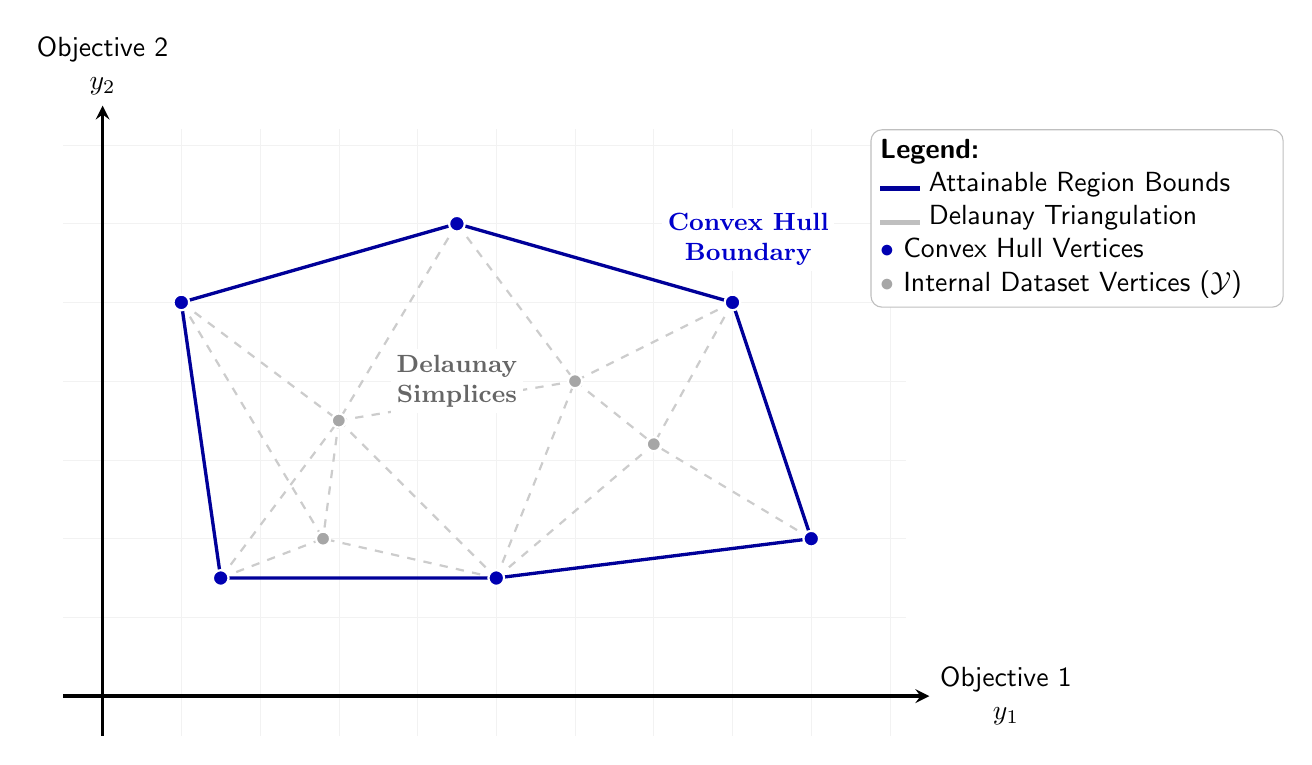
\begin{tikzpicture}[
    >=stealth,
    font=\sffamily,
    % Styles
    dataset_point/.style={circle, fill=gray!70, inner sep=1.8pt, draw=white, thick},
    hull_point/.style={circle, fill=blue!70!black, inner sep=2pt, draw=white, thick},
    mesh_edge/.style={gray!40, thick, dashed},
    hull_edge/.style={blue!60!black, very thick}
]

    % ==========================================
    % 1. BACKGROUND GRID & AXES
    % ==========================================
    \draw[step=1cm, gray!10, very thin] (-0.5, -0.5) grid (10.2, 7.2);
    \draw[->, very thick] (-0.5, 0) -- (10.5, 0) node[right, align=center] {Objective 1\\$y_1$};
    \draw[->, very thick] (0, -0.5) -- (0, 7.5) node[above, align=center] {Objective 2\\$y_2$};

    % ==========================================
    % 2. COORDINATES DEFINITION (Sparse Dataset Y)
    % ==========================================
    % Hull Vertices (The outer boundary)
    \coordinate (P1) at (1.0, 5.0);
    \coordinate (P2) at (1.5, 1.5);
    \coordinate (P4) at (4.5, 6.0);
    \coordinate (P5) at (5.0, 1.5);
    \coordinate (P7) at (8.0, 5.0);
    \coordinate (P8) at (9.0, 2.0);

    % Internal Vertices (A bunch of points)
    \coordinate (P3) at (3.0, 3.5);
    \coordinate (P6) at (6.0, 4.0);
    \coordinate (P9) at (2.8, 2.0);  % Added internal point
    \coordinate (P10) at (7.0, 3.2); % Added internal point

    % ==========================================
    % 3. DELAUNAY MESH EDGES (Internal)
    % ==========================================
    % Connecting the internal simplices
    \draw[mesh_edge] (P1) -- (P3);
    \draw[mesh_edge] (P4) -- (P3);
    \draw[mesh_edge] (P4) -- (P6);
    \draw[mesh_edge] (P7) -- (P6);
    
    % Connections to/from P9
    \draw[mesh_edge] (P1) -- (P9);
    \draw[mesh_edge] (P2) -- (P3);
    \draw[mesh_edge] (P2) -- (P9);
    \draw[mesh_edge] (P3) -- (P9);
    \draw[mesh_edge] (P5) -- (P9);
    \draw[mesh_edge] (P3) -- (P5);
    
    % Connections to/from P10
    \draw[mesh_edge] (P3) -- (P6);
    \draw[mesh_edge] (P5) -- (P6);
    \draw[mesh_edge] (P6) -- (P10);
    \draw[mesh_edge] (P7) -- (P10);
    \draw[mesh_edge] (P8) -- (P10);
    \draw[mesh_edge] (P5) -- (P10);

    % ==========================================
    % 4. CONVEX HULL (The currently attainable region)
    % ==========================================
    \draw[hull_edge] (P1) -- (P2) -- (P5) -- (P8) -- (P7) -- (P4) -- cycle;

    % ==========================================
    % 5. DRAW POINTS (Drawn last to overlay edges)
    % ==========================================
    % Internal Points
    \node[dataset_point] at (P3) {};
    \node[dataset_point] at (P6) {};
    \node[dataset_point] at (P9) {};
    \node[dataset_point] at (P10) {};
    
    % Hull Points
    \foreach \p in {P1, P2, P4, P5, P7, P8} {
        \node[hull_point] at (\p) {};
    }

    % ==========================================
    % 6. ANNOTATIONS
    % ==========================================
    % Convex Hull Label
    \node[text=blue!80!black, font=\bfseries\small, align=center, fill=white, inner sep=2pt] 
        at (8.2, 5.8) {Convex Hull\\Boundary};
        
    % Internal Mesh Label
    \node[text=gray!80!black, font=\bfseries\small, align=center, fill=white, inner sep=2pt] 
        at (4.5, 4.0) {Delaunay\\Simplices};

    % ==========================================
    % 7. LEGEND
    % ==========================================
    \node[draw=gray!50, fill=white, rounded corners, text width=5.0cm, align=left, anchor=north east] 
        at (15.0, 7.2) {
        \textbf{Legend:}\\
        \textcolor{blue!60!black}{\rule{0.5cm}{2pt}} Attainable Region Bounds\\
        \textcolor{gray!50}{\rule{0.5cm}{1.5pt}} Delaunay Triangulation\\
        \textcolor{blue!70!black}{$\bullet$} Convex Hull Vertices\\
        \textcolor{gray!70}{$\bullet$} Internal Dataset Vertices ($\mathcal{Y}$)
    };

\end{tikzpicture}